\documentclass[11pt,a4paper]{article}

\usepackage[utf8]{inputenc}
\usepackage[T1]{fontenc}
\usepackage[italian]{babel}
\usepackage{lmodern}
\usepackage[a4paper, margin=2cm, headheight=14pt]{geometry}
\usepackage{graphicx}
\usepackage{xcolor}
\usepackage{tikz}
\usepackage[most]{tcolorbox}
\usepackage{booktabs}
\usepackage{tabularx}
\usepackage{longtable}
\usepackage{array}
\usepackage{enumitem}
\usepackage{caption}
\usepackage{subcaption}
\usepackage{fancyhdr}
\usepackage{titlesec}
\usepackage{amssymb}
\usepackage{hyperref}

% Percorsi delle immagini esistenti nel progetto
\graphicspath{{../src/docs/img/}{../build/}}

% Palette colori (allineata a OpenflowDiagram)
\definecolor{ofPrimary}{HTML}{007AFF}
\definecolor{ofPrimaryLight}{HTML}{E6F1FF}
\definecolor{ofNoteBorder}{HTML}{C3DCFF}
\definecolor{ofNoteTitle}{HTML}{0060D1}
\definecolor{ofTipBg}{HTML}{E8F7EC}
\definecolor{ofTipBorder}{HTML}{BFE8CA}
\definecolor{ofTipTitle}{HTML}{1E8A3C}
\definecolor{ofText}{HTML}{1C1C1E}
\definecolor{ofMuted}{HTML}{6E6E73}
\definecolor{ofBorder}{HTML}{E3E3E8}
\definecolor{ofSurface}{HTML}{F7F7F9}
\definecolor{ofRed}{HTML}{FF3B30}
\definecolor{ofGreen}{HTML}{34C759}

\hypersetup{
  colorlinks=true,
  linkcolor=ofPrimary,
  urlcolor=ofPrimary,
  pdftitle={OpenflowDiagram - Guida introduttiva},
  pdfauthor={Francesco Gallo},
  pdfsubject={Programmare con i diagrammi di flusso}
}

% Intestazione e piè di pagina
\pagestyle{fancy}
\fancyhf{}
\lhead{\small\textcolor{ofMuted}{OpenflowDiagram 1.0.0}}
\rhead{\small\textcolor{ofMuted}{Guida introduttiva}}
\cfoot{\small\textcolor{ofMuted}{\thepage}}
\renewcommand{\headrulewidth}{0.4pt}

% Stile sezioni
\titleformat{\section}
  {\Large\bfseries\color{ofText}}
  {\colorbox{ofPrimary}{\makebox[1.4em][c]{\textcolor{white}{\thesection}}}}
  {0.6em}
  {}
\titleformat{\subsection}
  {\large\bfseries\color{ofText}}
  {}
  {0pt}
  {}

\captionsetup{font={small,color=ofMuted}, labelfont=bf}
\setlength{\parindent}{0pt}
\setlength{\parskip}{6pt}

% Comandi di utilità
\newcommand{\code}[1]{\colorbox{ofSurface}{\texttt{\small #1}}}
\newcommand{\kbd}[1]{\fcolorbox{ofBorder}{white}{\textsf{\footnotesize\bfseries #1}}}
\newcommand{\pill}[3]{\colorbox{#1}{\textcolor{#2}{\textsf{\footnotesize\bfseries #3}}}}
\newcommand{\nlbadge}[1]{\colorbox{ofGreen}{\textcolor{white}{\textsf{\footnotesize\bfseries #1}}}}
\newcommand{\menuarrow}{\,\textsf{\guilsinglright}\,}

% Box informativi
\newtcolorbox{notebox}{
  colback=ofPrimaryLight,
  colframe=ofNoteBorder,
  boxrule=0.8pt,
  arc=5pt,
  left=8pt, right=8pt, top=6pt, bottom=6pt,
  fonttitle=\bfseries\color{ofNoteTitle},
  title={Da sapere}
}

\newtcolorbox{tipbox}{
  colback=ofTipBg,
  colframe=ofTipBorder,
  boxrule=0.8pt,
  arc=5pt,
  left=8pt, right=8pt, top=6pt, bottom=6pt,
  fonttitle=\bfseries\color{ofTipTitle},
  title={Suggerimento}
}

\newtcolorbox{cardbox}[1]{
  colback=ofSurface,
  colframe=ofBorder,
  boxrule=0.6pt,
  arc=5pt,
  left=6pt, right=6pt, top=5pt, bottom=5pt,
  title={\textbf{\textcolor{ofPrimary}{#1}}},
  coltitle=ofPrimary,
  colbacktitle=ofSurface,
  boxed title style={empty},
  attach title to upper={\par\vspace{2pt}}
}

\begin{document}

% ==================== COPERTINA / HERO ====================
\begin{tcolorbox}[
  colback=ofPrimaryLight!40!white,
  colframe=ofBorder,
  boxrule=0.8pt,
  arc=8pt,
  left=14pt, right=14pt, top=14pt, bottom=14pt
]
\begin{minipage}[c]{0.15\linewidth}
  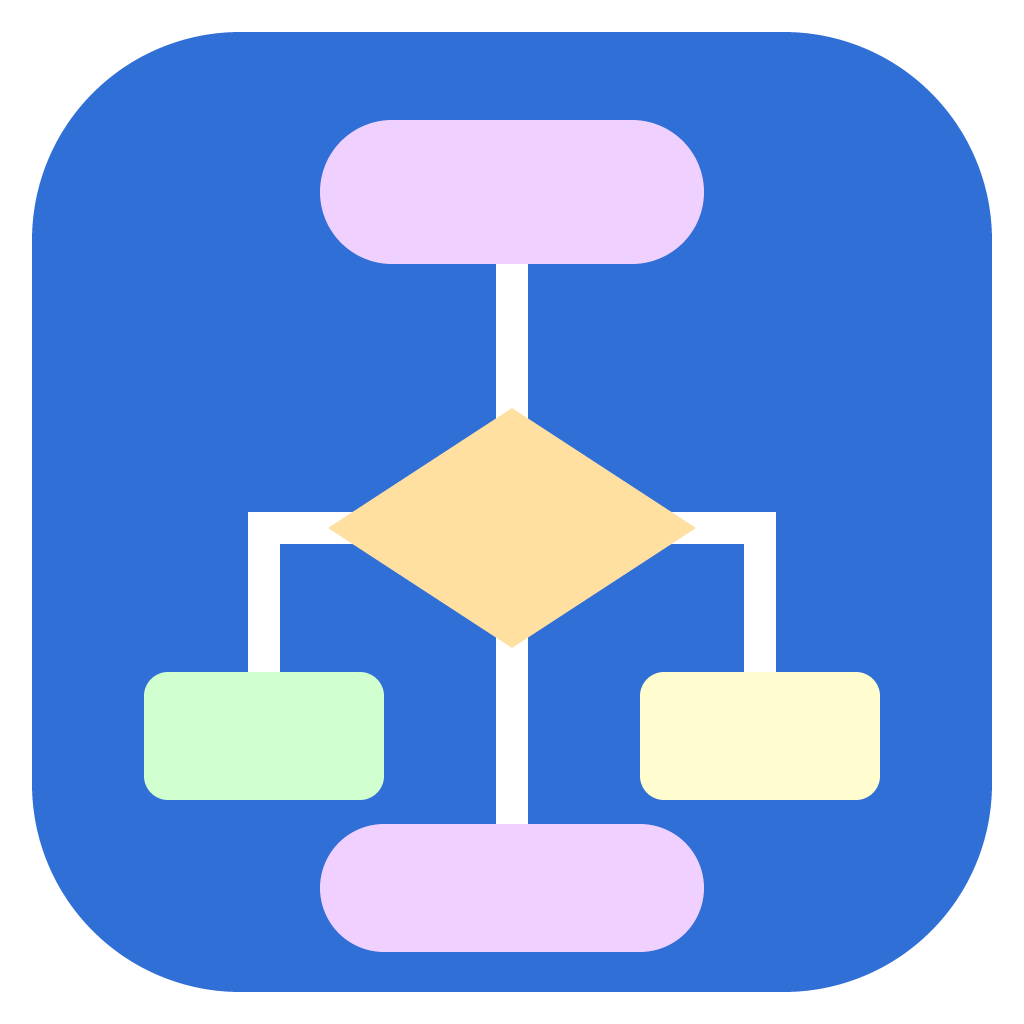
\includegraphics[width=\linewidth]{icon.png}
\end{minipage}\hfill
\begin{minipage}[c]{0.81\linewidth}
  {\footnotesize\bfseries\textcolor{ofPrimary}{\MakeUppercase{Guida introduttiva \textperiodcentered\ versione 1.0.0}}}\\[3pt]
  {\Large\bfseries Programmare con i diagrammi di flusso}\\[6pt]
  {\normalsize\textcolor{ofText}{Tutto quello che serve per usare OpenflowDiagram: creare un programma, eseguirlo passo passo, seguirne i valori con la tabella di traccia e tradurlo in C, C++, Java o Python.}}
\end{minipage}
\end{tcolorbox}

\tableofcontents
\vspace{1em}

% ==================== 1. BENVENUTO ====================
\section{Benvenuto in OpenflowDiagram}
OpenflowDiagram è un ambiente per imparare a programmare \textbf{disegnando}: invece di scrivere codice, costruisci un diagramma di flusso con blocchi grafici (dichiarazioni, input, output, condizioni, cicli\ldots) e lo esegui subito. Puoi:

\vspace{4pt}
\begin{minipage}[t]{0.48\linewidth}
  \begin{cardbox}{Costruire}
    Inserisci i blocchi cliccando sulle frecce del diagramma.
  \end{cardbox}
\end{minipage}\hfill
\begin{minipage}[t]{0.48\linewidth}
  \begin{cardbox}{Eseguire}
    Tutto insieme o un blocco alla volta, guardando le variabili cambiare.
  \end{cardbox}
\end{minipage}

\vspace{4pt}
\begin{minipage}[t]{0.48\linewidth}
  \begin{cardbox}{Tracciare}
    La tabella di traccia registra valori e condizioni a ogni passo.
  \end{cardbox}
\end{minipage}\hfill
\begin{minipage}[t]{0.48\linewidth}
  \begin{cardbox}{Tradurre}
    Il diagramma diventa codice C, C++, Java o Python, sempre aggiornato.
  \end{cardbox}
\end{minipage}

\begin{notebox}
I programmi si salvano in file \code{.fprg}, lo stesso formato di Flowgorithm: puoi aprire i file creati con Flowgorithm e viceversa (per i blocchi supportati).
\end{notebox}

% ==================== 2. LA FINESTRA PRINCIPALE ====================
\section{La finestra principale}
All'avvio OpenflowDiagram mostra un programma vuoto. Questa è la finestra con un programma d'esempio appena eseguito:

\begin{figure}[htbp]
  \centering
  \begin{tikzpicture}
    \node[anchor=south west, inner sep=0] (img) at (0,0) {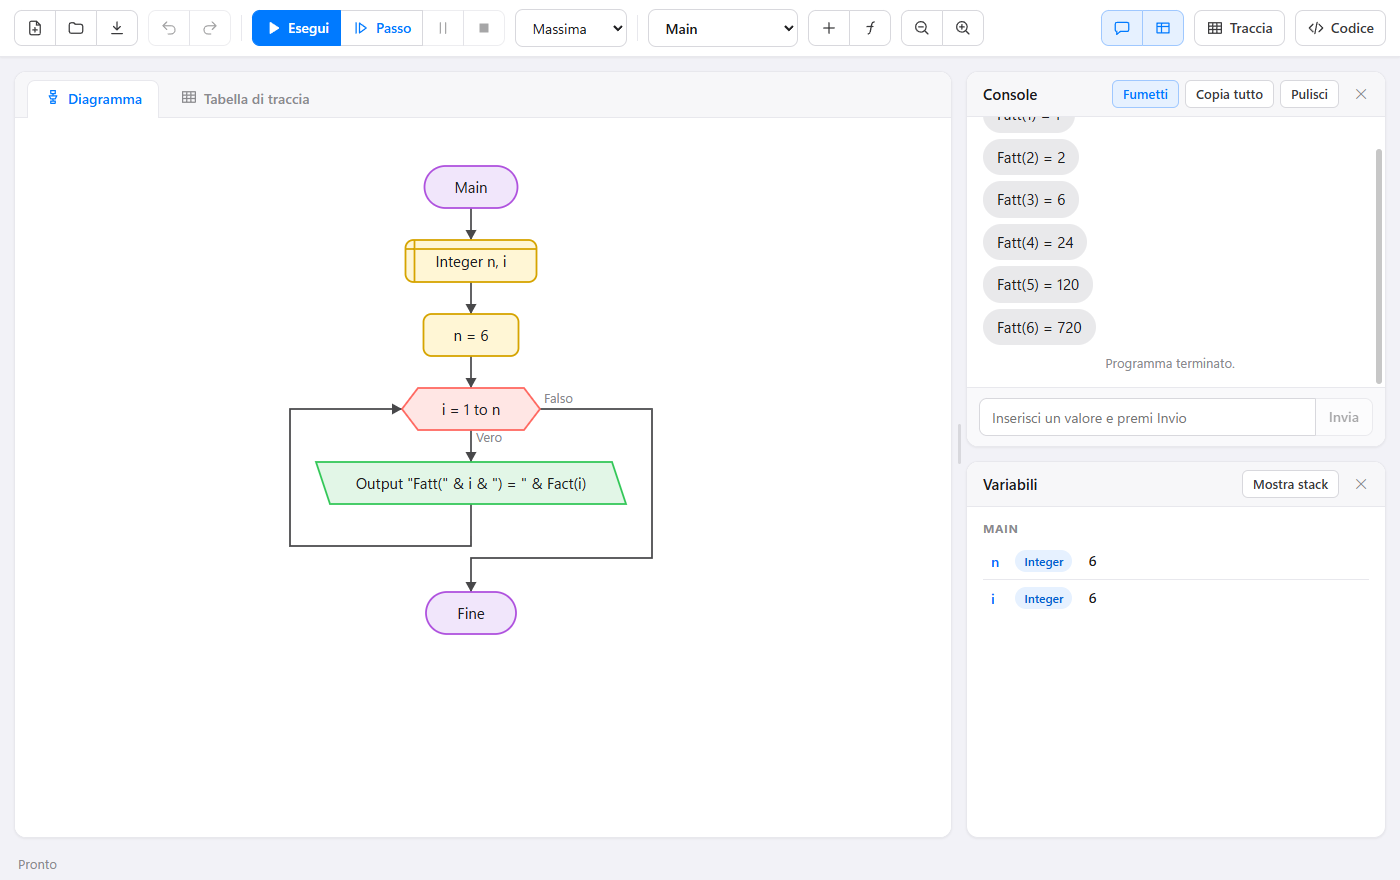
\includegraphics[width=\linewidth]{overview.png}};
    \begin{scope}[x={(img.south east)}, y={(img.north west)}]
      \tikzset{badge/.style={circle, fill=ofRed, text=white, draw=white, line width=1.2pt, font=\scriptsize\bfseries, inner sep=1.5pt, minimum size=15pt}}
      \node[badge] at (0.0471, 0.9318) {1};
      \node[badge] at (0.2391, 0.9318) {2};
      \node[badge] at (0.3628, 0.9307) {3};
      \node[badge] at (0.4496, 0.9307) {4};
      \node[badge] at (0.2929, 0.8966) {5};
      \node[badge] at (0.0421, 0.8205) {6};
      \node[badge] at (0.6886, 0.7089) {7};
      \node[badge] at (0.6886, 0.2632) {8};
      \node[badge] at (0.9479, 0.9318) {9};
      \node[badge] at (0.9793, 0.9318) {10};
    \end{scope}
  \end{tikzpicture}
  \caption{La finestra principale di OpenflowDiagram.}
\end{figure}

\begin{enumerate}[label=\textbf{\arabic*.}, leftmargin=2em, itemsep=2pt]
  \item File: nuovo, apri, salva
  \item Esegui, Passo, Pausa, Ferma
  \item Velocità di esecuzione
  \item Funzione mostrata nel diagramma
  \item Schede Diagramma e Tabella di traccia
  \item Il diagramma di flusso
  \item Console: output e input
  \item Variabili e loro valori
  \item Tabella di traccia
  \item Finestra del codice sorgente
\end{enumerate}

La \textbf{barra dei menu} (File, Modifica, Programma, Visualizza, Strumenti, Aiuto) contiene tutti i comandi, anche quelli che non hanno un pulsante. Console e Variabili si possono chiudere con la \kbd{$\times$} e riaprire con i pulsanti a destra della barra; il bordo tra diagramma e pannelli si trascina per cambiarne la larghezza.

% ==================== 3. IL PRIMO PROGRAMMA ====================
\section{Il primo programma}
Costruiamo un programma che chiede il nome e saluta: \textit{``Come ti chiami?'' $\rightarrow$ Ada $\rightarrow$ ``Ciao, Ada!''}

\subsection{1. Inserisci un blocco}
Un programma nuovo contiene solo \textbf{Main} e \textbf{Fine}. Clicca sulla \textbf{freccia} tra i due: si apre il menu dei blocchi, diviso in Blocchi, Cicli, Altro e File. Ogni pulsante mostra la forma del blocco.

\begin{figure}[htbp]
  \centering
  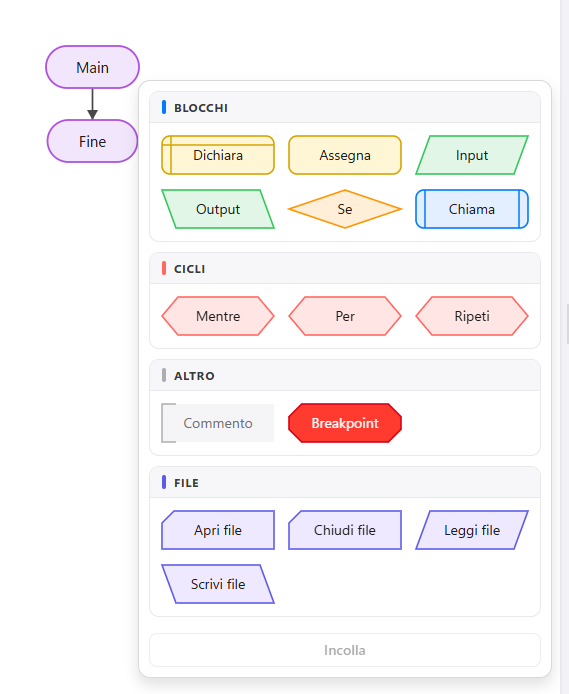
\includegraphics[width=0.92\linewidth]{tutorial-insert.png}
  \caption{Il menu che compare cliccando su una freccia.}
\end{figure}

\subsection{2. Dichiara una variabile}
Scegli \textbf{Dichiara}. Nella finestra scrivi il nome \code{nome} e scegli il tipo \textbf{String}, poi \textbf{OK}. Le variabili vanno sempre dichiarate prima di usarle.

\begin{figure}[htbp]
  \centering
  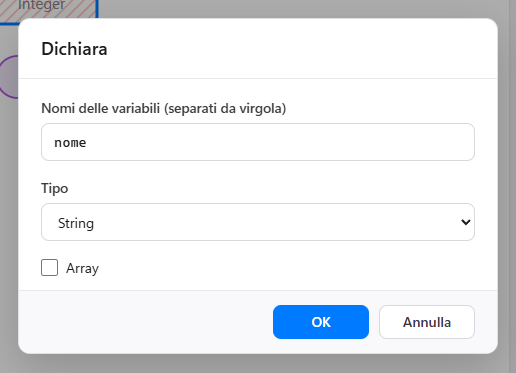
\includegraphics[width=0.62\linewidth]{tutorial-declare.png}
  \caption{La finestra del blocco Dichiara.}
\end{figure}

\subsection{3. Aggiungi Output e Input}
Clicca sulla freccia sotto \textit{String nome} e scegli \textbf{Output}: scrivi \code{"Come ti chiami?"} (il testo va tra virgolette). Poi, sotto, un blocco \textbf{Input} con la variabile \code{nome}, e infine un altro \textbf{Output} con \code{"Ciao, " \& nome \& "!"} --- il simbolo \code{\&} unisce testi e valori.

\begin{figure}[htbp]
  \centering
  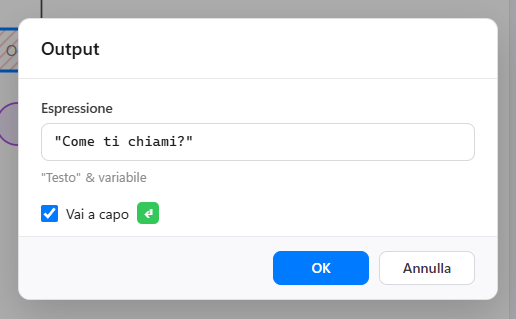
\includegraphics[width=0.62\linewidth]{tutorial-output.png}
  \caption{La finestra del blocco Output: l'opzione ``Vai a capo'' è attiva di default.}
\end{figure}

\begin{tipbox}
Nel diagramma ogni Output mostra \nlbadge{$\hookleftarrow$} se va a capo e \nlbadge{$\rightarrow$} se il testo successivo continua sulla stessa riga: utile per stampare più valori uno accanto all'altro.
\end{tipbox}

\subsection{4. Controlla il diagramma}
Il programma completo è questo. Se un campo è vuoto o un'espressione è sbagliata, OpenflowDiagram te lo dice subito nella finestra del blocco; un blocco lasciato vuoto appare tratteggiato.

\begin{figure}[htbp]
  \centering
  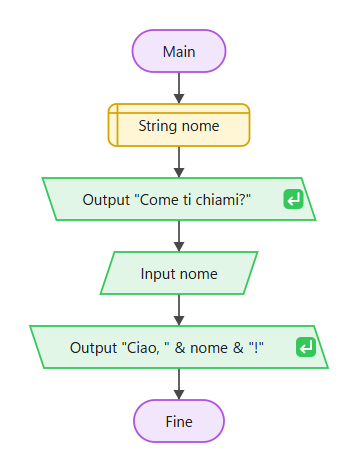
\includegraphics[width=0.58\linewidth]{tutorial-chart.png}
  \caption{Il programma ``Saluto''.}
\end{figure}

\subsection{5. Esegui e rispondi}
Premi \textbf{Esegui} (\kbd{F5}). Quando il programma arriva al blocco Input, la casella in fondo alla Console si illumina: scrivi la risposta e premi \kbd{Invio}.

\begin{figure}[htbp]
  \centering
  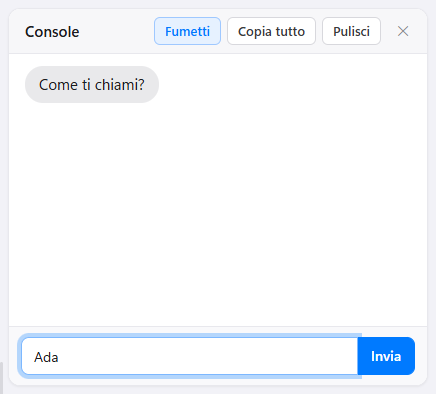
\includegraphics[width=0.62\linewidth]{tutorial-waiting.png}
  \caption{La Console attende un valore.}
\end{figure}

\begin{figure}[htbp]
  \centering
  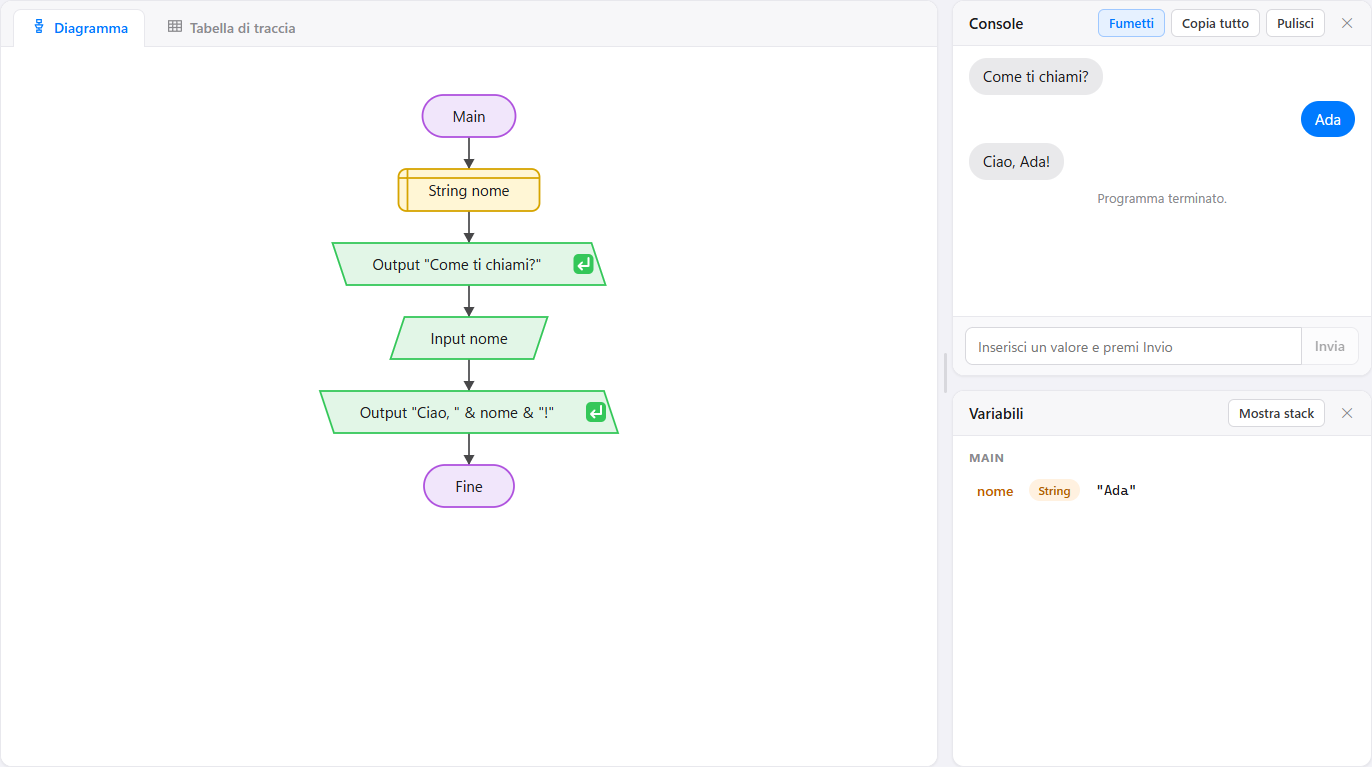
\includegraphics[width=0.92\linewidth]{tutorial-run.png}
  \caption{Il programma terminato: l'output nella Console e il valore di \code{nome} nel pannello Variabili.}
\end{figure}

\subsection{6. Salva}
Usa \textbf{File \menuarrow{} Salva} (\kbd{Ctrl}+\kbd{S}). Il pallino \textbullet\ nel titolo della finestra indica modifiche non salvate.

% ==================== 4. I BLOCCHI ====================
\section{I blocchi}
\begin{longtable}{>{\bfseries}p{2.4cm} p{7.6cm} p{5.5cm}}
  \toprule
  Blocco & A cosa serve & Esempio \\
  \midrule
  \endhead
  \bottomrule
  \endfoot
  Dichiara & Crea una o più variabili di un tipo (Integer, Real, String, Boolean), anche come array. & \code{Integer n, i} \textperiodcentered\ \code{Real Array voti[10]} \\
  Assegna & Calcola un'espressione e ne mette il risultato in una variabile. & \code{somma = somma + x} \\
  Input & Chiede un valore all'utente nella Console e lo salva in una variabile. & \code{Input nome} \\
  Output & Mostra un valore o un testo nella Console. Il simbolo nel blocco indica se poi \textbf{va a capo} (\nlbadge{$\hookleftarrow$}) o se il prossimo output \textbf{continua sulla stessa riga} (\nlbadge{$\rightarrow$}). & \code{Output "Ciao, " \& nome} \\
  Se & Sceglie tra due rami in base a una condizione: Vero a destra, Falso a sinistra. & \code{Se voto >= 6} \\
  Chiama & Esegue una funzione che non restituisce valori. & \code{Ordina(v)} \\
  Mentre & Ripete il corpo finché la condizione è vera (controllo all'inizio). & \code{Mentre n != 1} \\
  Per & Ripete con un contatore da un valore iniziale a uno finale, crescente o decrescente, con passo. & \code{Per i = 1 to 10 step 2} \\
  Ripeti & Esegue il corpo almeno una volta e lo ripete finché la condizione è vera (controllo alla fine). & \code{Ripeti \ldots\ mentre risposta != "no"} \\
  Commento & Una nota nel diagramma: non viene eseguita. & \code{Calcolo della media} \\
  Breakpoint & Mette in pausa l'esecuzione in quel punto (sempre o solo se una condizione è vera). & \code{Breakpoint: i == 5} \\
  Apri file & Apre un file di testo in lettura o in scrittura. & \code{Apri file "dati.txt" (Lettura)} \\
  Leggi file & Legge la riga successiva del file in una variabile. & \code{Leggi file x} \\
  Scrivi file & Scrive un valore come nuova riga del file. & \code{Scrivi file totale} \\
  Chiudi file & Chiude il file aperto (i dati scritti vengono salvati). & \code{Chiudi file} \\
\end{longtable}

\subsection{Lavorare con i blocchi}
\begin{itemize}[label=\textcolor{ofPrimary}{$\checkmark$}, leftmargin=1.8em]
  \item \textbf{Modificare}: doppio clic sul blocco (oppure selezionalo e premi \kbd{Invio}).
  \item \textbf{Selezionare più blocchi}: clic sul primo e \kbd{Shift}+clic sull'ultimo (devono essere nello stesso ramo).
  \item \textbf{Tagliare, copiare, incollare, eliminare}: clic destro sul blocco, oppure \kbd{Ctrl}+\kbd{X}/\kbd{C}/\kbd{V} e \kbd{Canc}. Per incollare in un punto preciso, clicca la freccia e scegli \textbf{Incolla} in fondo al menu.
  \item \textbf{Annullare}: \kbd{Ctrl}+\kbd{Z} e \kbd{Ctrl}+\kbd{Y} annullano e ripetono qualsiasi modifica.
  \item \textbf{Zoom}: pulsanti lente nella barra, oppure \kbd{Ctrl}+rotellina.
\end{itemize}

\begin{figure}[htbp]
  \centering
  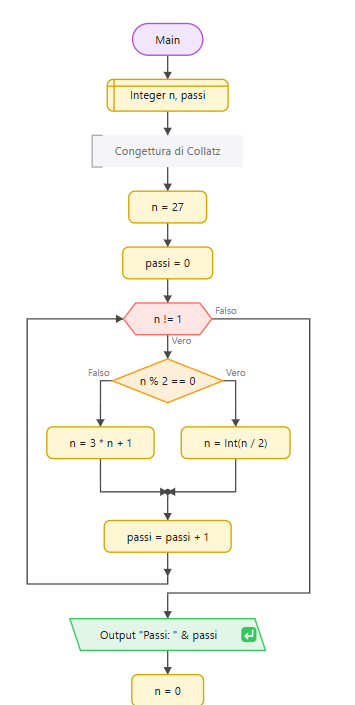
\includegraphics[width=0.62\linewidth]{shapes.png}
  \caption{Se e cicli: il ramo Vero e il ramo Falso, e la freccia che riporta all'inizio del ciclo Mentre (esempio ``Cicli'').}
\end{figure}

% ==================== 5. TIPI, OPERATORI E FUNZIONI ====================
\section{Tipi, operatori e funzioni}

\subsection{Tipi}
\begin{tabularx}{\linewidth}{l X}
  \toprule
  \textbf{Tipo} & \textbf{Valori} \\
  \midrule
  \pill{ofPrimaryLight}{ofNoteTitle}{Integer} & numeri interi: \code{42}, \code{-7} \\
  \pill{purple!12}{purple!80!black}{Real} & numeri con la virgola: \code{3.14} \\
  \pill{orange!15}{orange!70!black}{String} & testo: \code{"ciao"} \\
  \pill{ofTipBg}{ofTipTitle}{Boolean} & \code{true} o \code{false} \\
  \bottomrule
\end{tabularx}

\subsection{Operatori}
\begin{tabularx}{\linewidth}{l X}
  \toprule
  \textbf{Operatore} & \textbf{Significato} \\
  \midrule
  \code{+ - * /} & aritmetica (\code{/} dà sempre un Real: \code{7 / 2 = 3.5}) \\
  \code{\%} o \code{mod} & resto della divisione \\
  \code{\^{}} & potenza: \code{2 \^{} 10} \\
  \code{\&} & unisce testi e valori \\
  \code{== != < <= > >=} & confronti (anche \code{=} e \code{<>}) \\
  \code{and or not} & logica (anche \code{\&\& || !}) \\
  \bottomrule
\end{tabularx}

\subsection{Funzioni predefinite}
\begin{longtable}{l p{10.5cm}}
  \toprule
  \textbf{Funzione} & \textbf{Risultato} \\
  \midrule
  \endhead
  \bottomrule
  \endfoot
  \code{Abs(x)} & valore assoluto \\
  \code{Sqrt(x)} & radice quadrata \\
  \code{Int(x)} & parte intera (tronca i decimali) \\
  \code{Sgn(x)} & segno: $-1$, $0$ o $1$ \\
  \code{Random(n)} & numero intero casuale da $0$ a $n-1$ \\
  \code{Log(x), Log10(x)} & logaritmo naturale e in base $10$ \\
  \code{Sin, Cos, Tan(x)} & funzioni trigonometriche (radianti) \\
  \code{ArcSin, ArcCos, ArcTan(x)} & funzioni inverse \\
  \code{Len(s)} & lunghezza di una stringa \\
  \code{Char(s, i)} & carattere in posizione $i$ (da $0$) \\
  \code{ToCode(s)} & codice del primo carattere \\
  \code{ToChar(n)} & carattere con codice $n$ \\
  \code{ToInteger(x)} & converte in Integer (anche da testo) \\
  \code{ToReal(x)} & converte in Real \\
  \code{ToString(x)} & converte in testo \\
  \code{ToFixed(x, d)} & testo con $d$ cifre decimali \\
  \code{Size(a)} & numero di elementi di un array \\
  \code{EOF()} & vero se il file aperto in lettura è finito \\
  \code{Pi} & la costante $\pi$ \\
\end{longtable}

\begin{tipbox}
Non serve ricordare i nomi: nelle finestre dei blocchi, accanto a ogni campo con un'espressione, il pulsante \textbf{\textit{f(x)}} apre l'elenco delle funzioni predefinite e delle tue funzioni, con una ricerca. Un clic inserisce la funzione nel punto in cui stai scrivendo, con il cursore già tra le parentesi.
\end{tipbox}

\begin{figure}[htbp]
  \centering
  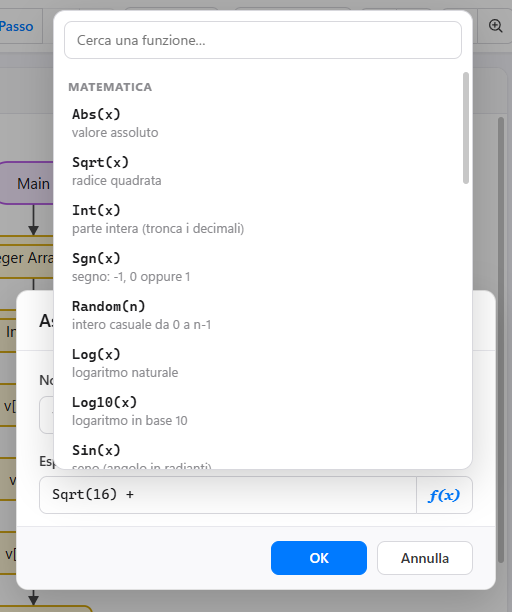
\includegraphics[width=0.62\linewidth]{function-picker.png}
  \caption{Il pulsante \textit{f(x)} nella finestra di un blocco Assegna.}
\end{figure}

\begin{notebox}
Gli array partono da $0$: un \code{Integer Array v[5]} ha gli elementi \code{v[0]} \ldots\ \code{v[4]}. Maiuscole e minuscole nei nomi non contano (\code{Somma} e \code{somma} sono la stessa variabile).
\end{notebox}

% ==================== 6. ESEGUIRE E FARE DEBUG ====================
\section{Eseguire e fare debug}
\begin{tabularx}{\linewidth}{l X}
  \toprule
  \textbf{Pulsante} & \textbf{Cosa fa} \\
  \midrule
  \textbf{Esegui} \kbd{F5} & Esegue il programma alla velocità scelta; durante una pausa, riprende. \\
  \textbf{Passo} \kbd{F10} & Esegue \textbf{un blocco alla volta}: il blocco evidenziato in arancione è quello che sta per essere eseguito. \\
  \textbf{Pausa} \kbd{F6} & Ferma temporaneamente un programma in esecuzione. \\
  \textbf{Ferma} \kbd{Shift}+\kbd{F5} & Interrompe il programma. \\
  \textbf{Velocità} & Lenta, Media, Veloce (per seguire l'evidenziazione) o Massima (risultato immediato). \\
  \bottomrule
\end{tabularx}

\begin{figure}[htbp]
  \centering
  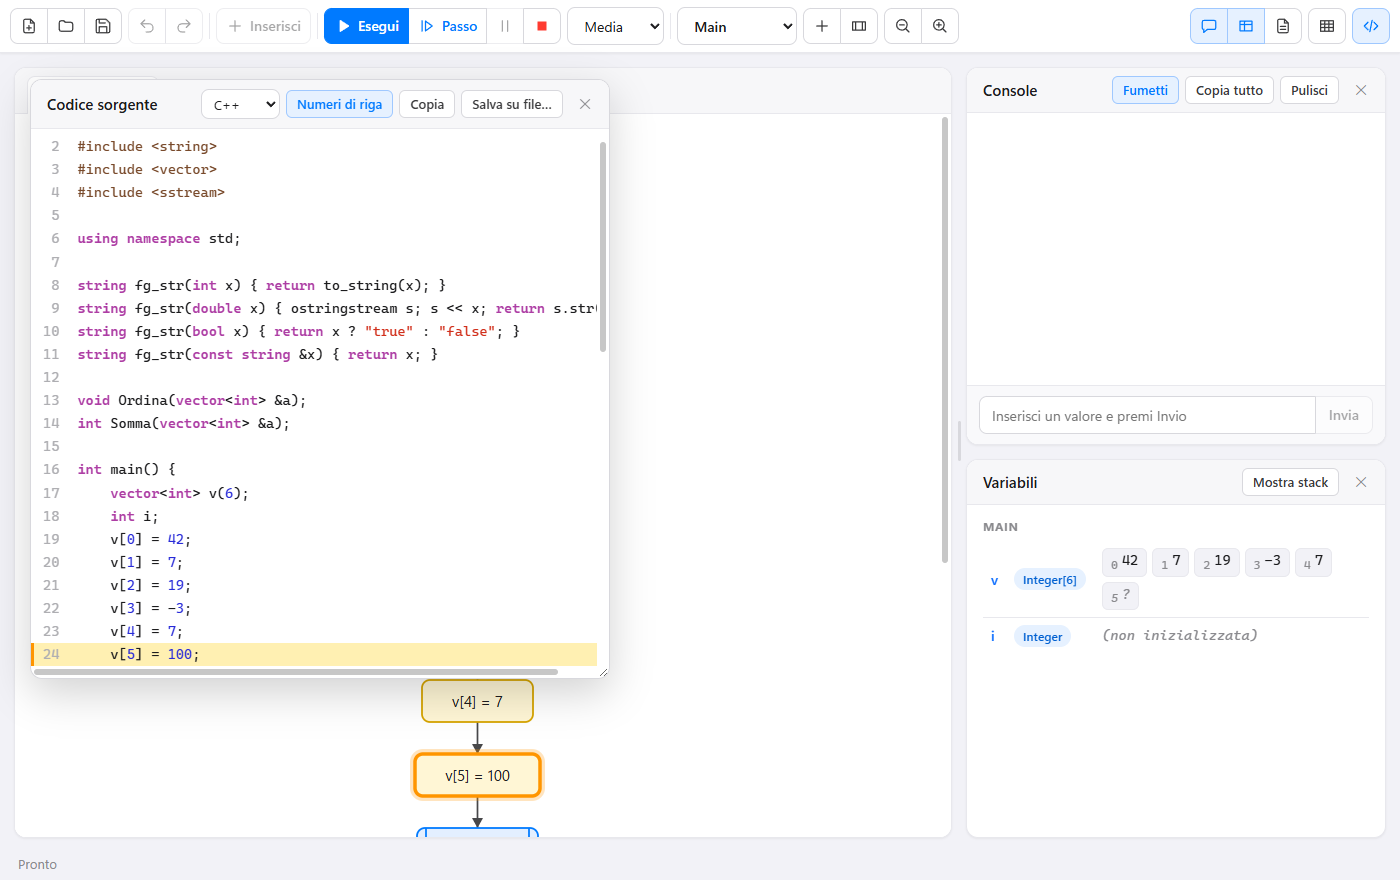
\includegraphics[width=0.95\linewidth]{step.png}
  \caption{Passo passo: il blocco evidenziato, la riga corrispondente nel codice e le variabili aggiornate.}
\end{figure}

\subsection{Breakpoint}
Un blocco \textbf{Breakpoint} mette in pausa il programma quando viene raggiunto (sempre, oppure solo se una condizione è vera). Da lì puoi continuare con \textbf{Esegui} o con \textbf{Passo}. \textbf{Programma \menuarrow{} Ignora i breakpoint} li salta tutti, \textbf{Rimuovi tutti i breakpoint} li elimina.

\begin{figure}[htbp]
  \centering
  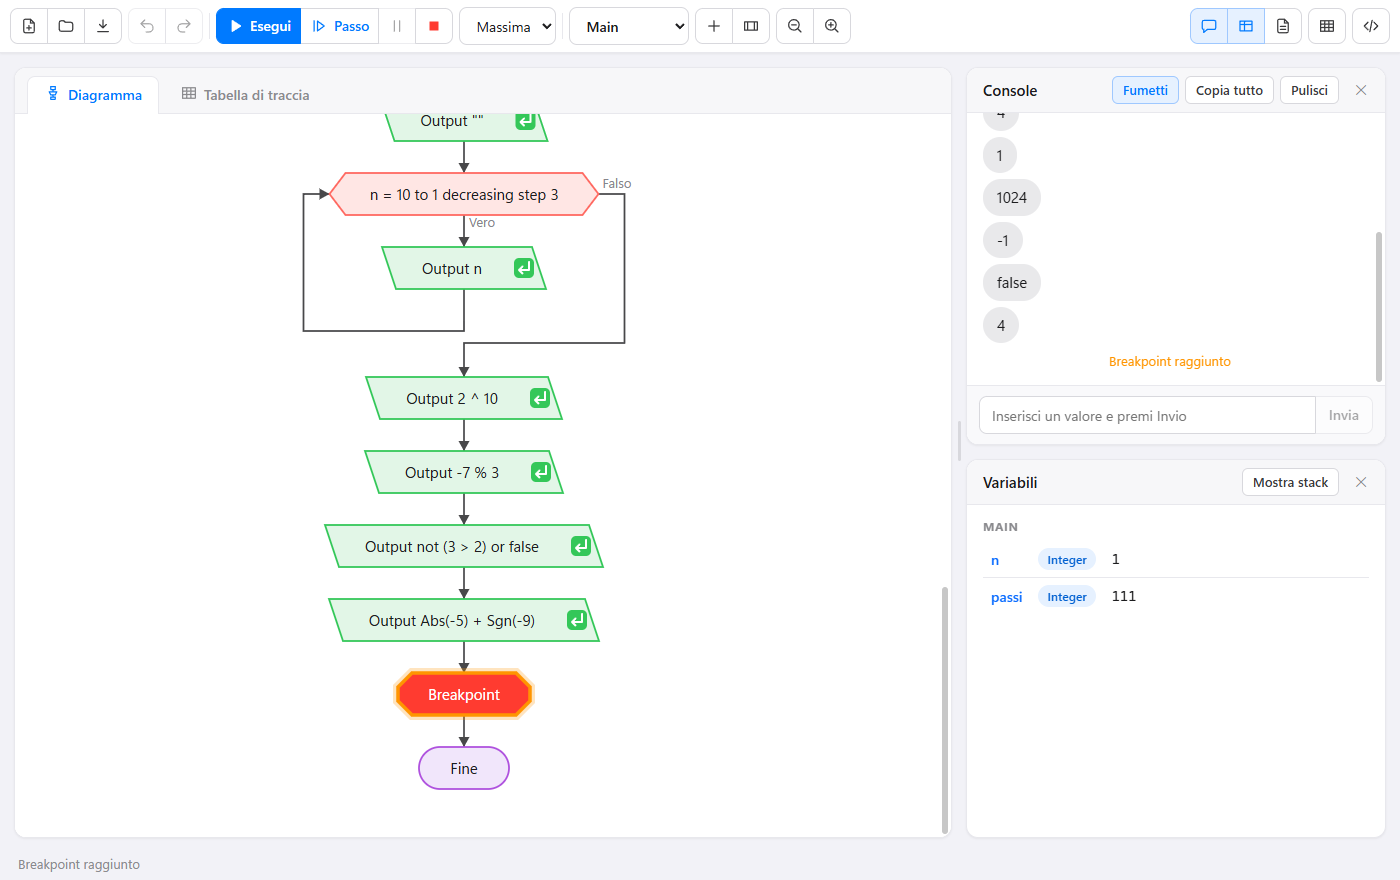
\includegraphics[width=0.95\linewidth]{breakpoint.png}
  \caption{Il programma in pausa sul breakpoint.}
\end{figure}

\subsection{Errori}
Se qualcosa va storto (divisione per zero, variabile non inizializzata, indice fuori dall'array\ldots) OpenflowDiagram si ferma, evidenzia in rosso il blocco responsabile e spiega il problema in italiano.

\begin{figure}[htbp]
  \centering
  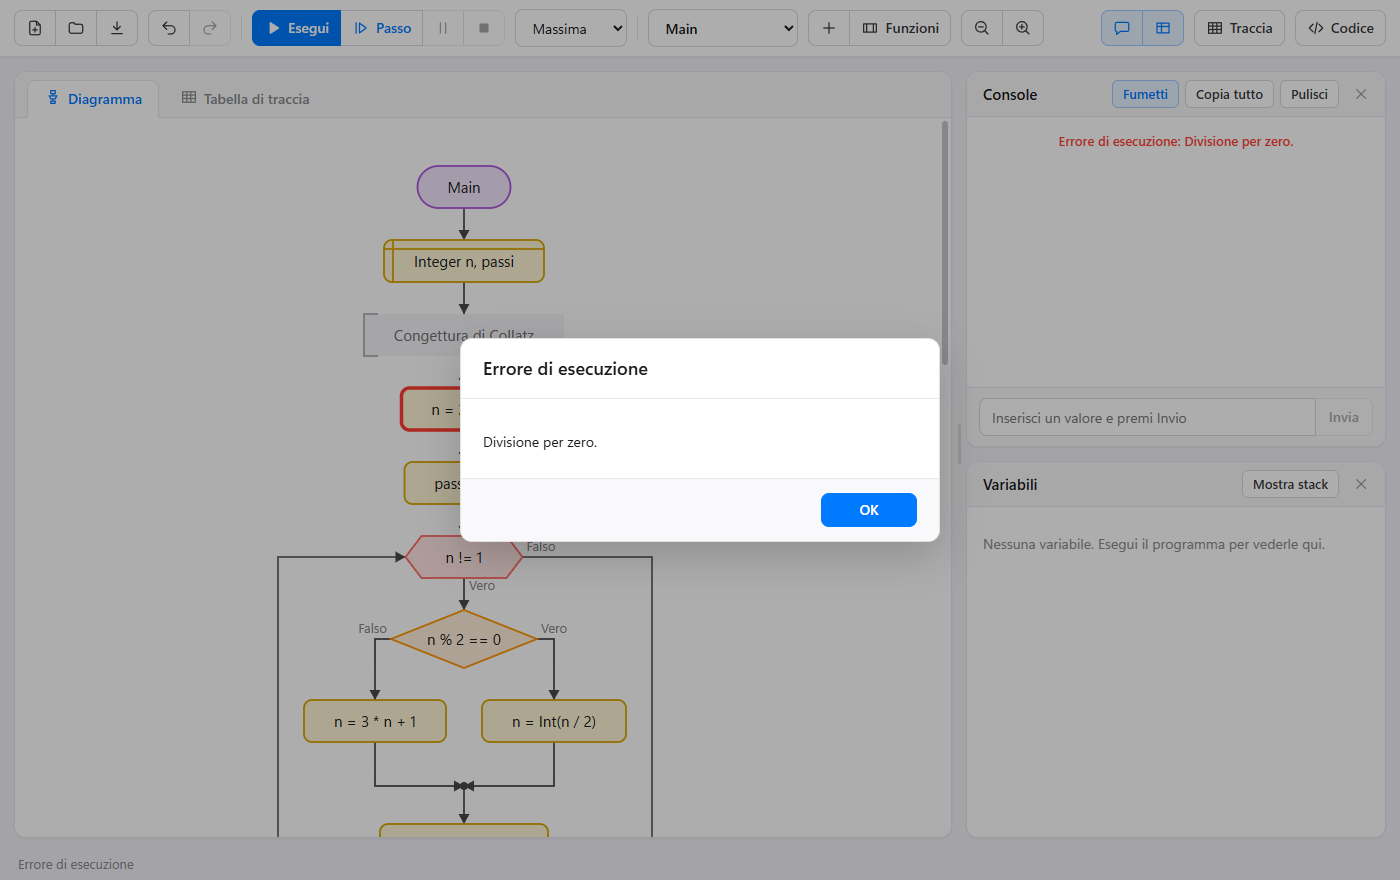
\includegraphics[width=0.95\linewidth]{error.png}
  \caption{Un errore di esecuzione: il blocco \code{n = 27 / 0} è evidenziato in rosso.}
\end{figure}

% ==================== 7. CONSOLE E VARIABILI ====================
\section{Console e Variabili}
La \textbf{Console} mostra l'output e raccoglie l'input. Con \textbf{Fumetti} attivo i messaggi appaiono come in una chat (programma a sinistra, tu a destra); disattivandolo diventa un terminale classico. \textbf{Copia tutto} copia il contenuto, \textbf{Pulisci} lo svuota.

Il pannello \textbf{Variabili} mostra il valore di ogni variabile mentre il programma gira; \code{?} indica una variabile non ancora inizializzata. Con \textbf{Mostra stack} vedi anche le variabili delle funzioni chiamanti:

\begin{figure}[htbp]
  \centering
  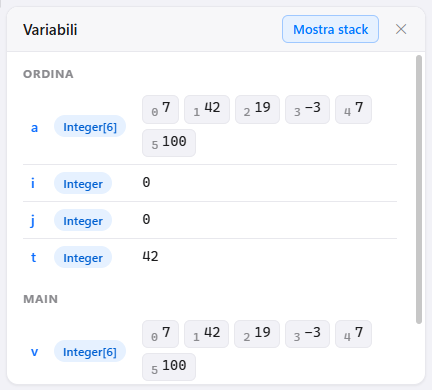
\includegraphics[width=0.62\linewidth]{variables-stack.png}
  \caption{Dentro la funzione Ordina: le sue variabili e, sotto, quelle di Main.}
\end{figure}

% ==================== 8. FUNZIONI ====================
\section{Funzioni}
Un programma può avere, oltre a \textbf{Main}, altre funzioni. Usa il pulsante \textbf{+} della barra (o \textbf{Programma \menuarrow{} Aggiungi funzione}) e scegli nome, tipo restituito, variabile restituita e parametri. Il menu a tendina nella barra mostra la funzione da modificare.

\begin{figure}[htbp]
  \centering
  \begin{subfigure}[t]{0.48\linewidth}
    \centering
    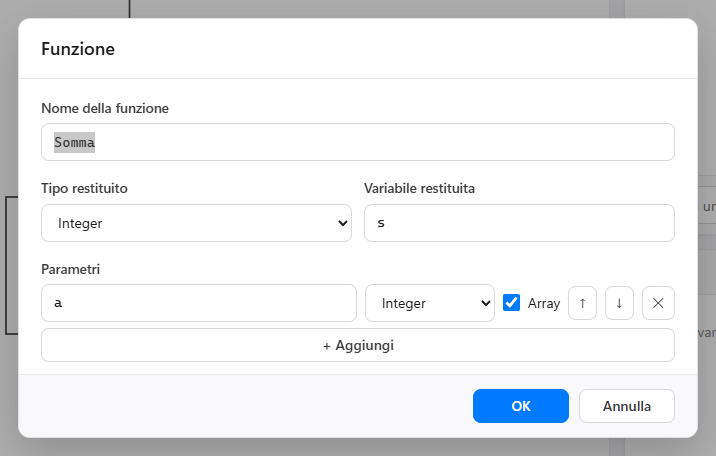
\includegraphics[width=\linewidth]{function-edit.png}
    \caption{Definizione di una funzione con un parametro array.}
  \end{subfigure}\hfill
  \begin{subfigure}[t]{0.48\linewidth}
    \centering
    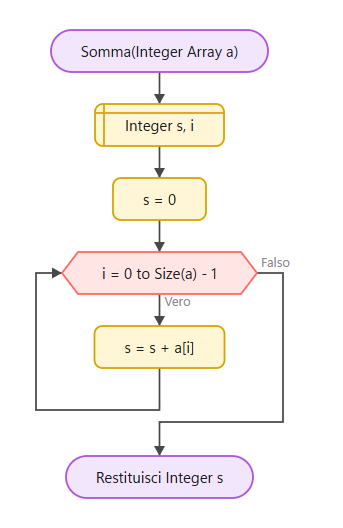
\includegraphics[width=\linewidth]{function-chart.png}
    \caption{Il diagramma della funzione Somma: il blocco finale restituisce \code{s}.}
  \end{subfigure}
\end{figure}

\begin{itemize}[label=\textcolor{ofPrimary}{$\checkmark$}, leftmargin=1.8em]
  \item Una funzione che restituisce un valore si usa nelle espressioni: \code{"Somma = " \& Somma(v)}.
  \item Una funzione senza valore (tipo \textbf{Nessuno}) si esegue con il blocco \textbf{Chiama}.
  \item I parametri normali ricevono una copia del valore; gli \textbf{array} sono passati per riferimento (la funzione può modificarli).
  \item Doppio clic sul blocco iniziale di una funzione per modificarne la definizione.
\end{itemize}

\begin{figure}[htbp]
  \centering
  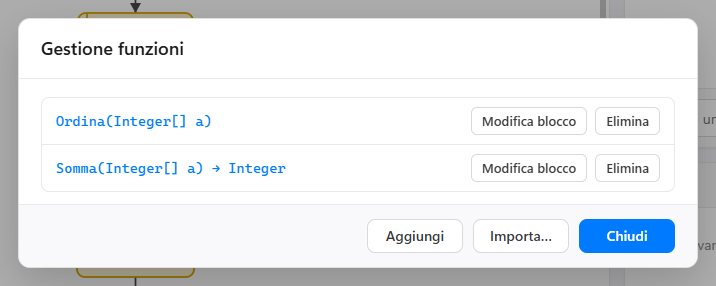
\includegraphics[width=0.62\linewidth]{functions-manager.png}
  \caption{\textbf{Gestione funzioni} (pulsante \textbf{Funzioni} nella barra): apri, modifica, elimina o importa funzioni da un altro file \code{.fprg}.}
\end{figure}

% ==================== 9. CODICE SORGENTE ====================
\section{Codice sorgente}
Il pulsante \textbf{Codice} (\kbd{F4}) apre una finestra mobile con il programma tradotto in \textbf{C, C++, Java o Python}. La traduzione si aggiorna mentre modifichi il diagramma e, durante l'esecuzione, evidenzia la riga del blocco corrente. Trascina la finestra dal titolo e ridimensionala dall'angolo in basso a destra.

\begin{figure}[htbp]
  \centering
  \begin{subfigure}[t]{0.48\linewidth}
    \centering
    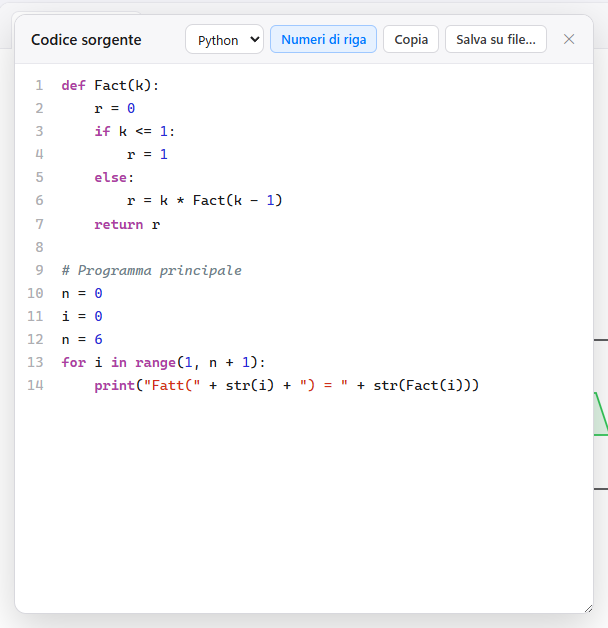
\includegraphics[width=\linewidth]{code-window.png}
    \caption{Il programma Fattoriale in Python.}
  \end{subfigure}\hfill
  \begin{subfigure}[t]{0.48\linewidth}
    \centering
    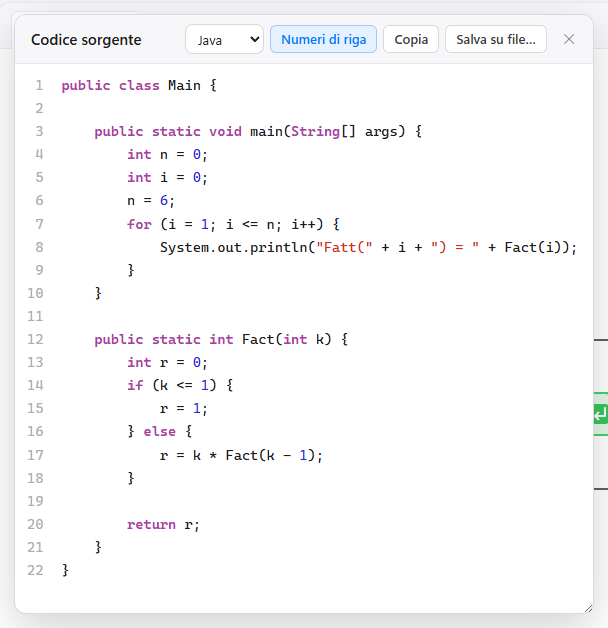
\includegraphics[width=\linewidth]{code-java.png}
    \caption{Lo stesso programma in Java.}
  \end{subfigure}
\end{figure}

\begin{tipbox}
\textbf{Copia} mette il codice negli appunti, \textbf{Salva su file\ldots} lo salva con l'estensione giusta (\code{.c}, \code{.cpp}, \code{.java}, \code{.py}), pronto da compilare o eseguire.
\end{tipbox}

% ==================== 10. TABELLA DI TRACCIA ====================
\section{Tabella di traccia}
La \textbf{tabella di traccia} è il modo classico per capire cosa fa un algoritmo: una riga per ogni blocco eseguito, con i valori delle variabili e l'esito delle condizioni. Si apre con il pulsante \textbf{Traccia} (\kbd{F7}) e compare in una scheda accanto al diagramma.

\subsection{1. Scegli cosa tracciare}
La prima volta OpenflowDiagram chiede quali \textbf{variabili} seguire (raggruppate per funzione) e quali \textbf{espressioni o condizioni} calcolare a ogni passo, per esempio \code{i \% 2 == 0}. Puoi cambiare la scelta con \textbf{Scegli valori\ldots}.

\begin{figure}[htbp]
  \centering
  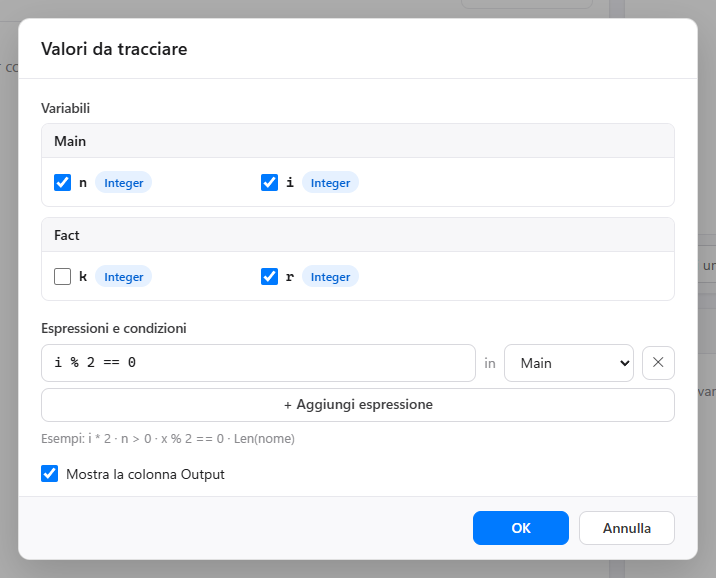
\includegraphics[width=0.62\linewidth]{trace-setup.png}
  \caption{La scelta dei valori: variabili di Main, la variabile \code{r} della funzione Fact e una condizione.}
\end{figure}

\subsection{2. Costruiscila passo passo}
Premi \textbf{Passo}: a ogni blocco eseguito si aggiunge una riga, e l'ultima è evidenziata. I valori appena cambiati sono in giallo, le condizioni mostrano \pill{ofTipBg}{ofTipTitle}{Vero} o \pill{red!12}{red!75!black}{Falso}.

\begin{figure}[htbp]
  \centering
  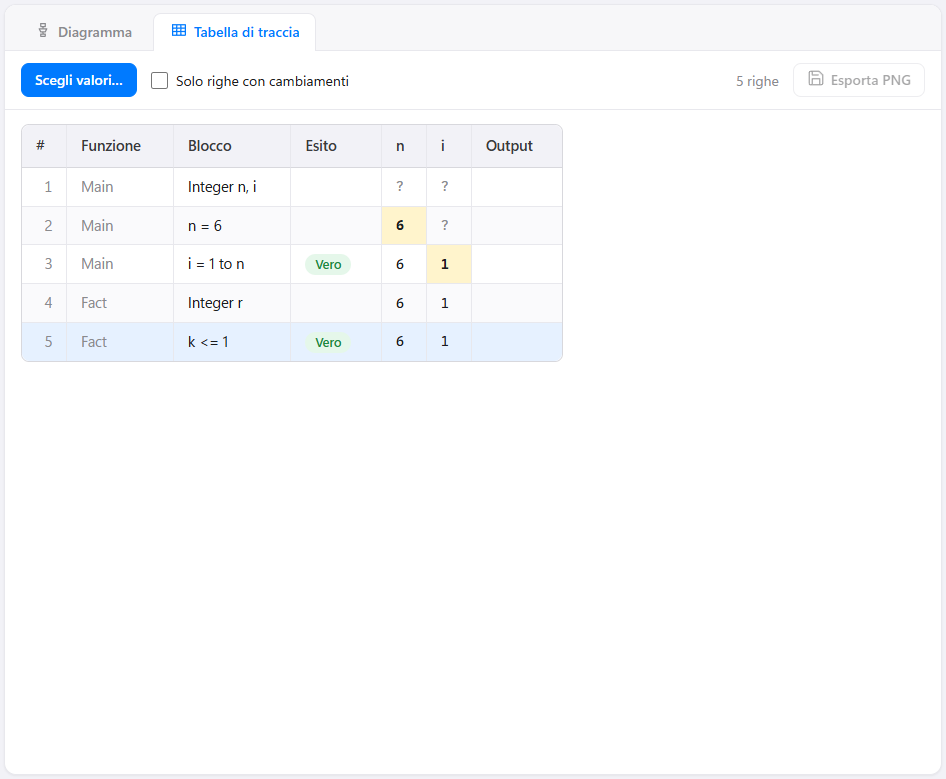
\includegraphics[width=0.95\linewidth]{trace-step.png}
  \caption{Dopo alcuni passi.}
\end{figure}

\subsection{3. Completa ed esporta}
Con \textbf{Esegui} la tabella si completa. \textbf{Solo righe con cambiamenti} nasconde le righe in cui non cambia nulla; \textbf{Esporta PNG} salva un'immagine della tabella, ideale per consegne e appunti.

\begin{figure}[htbp]
  \centering
  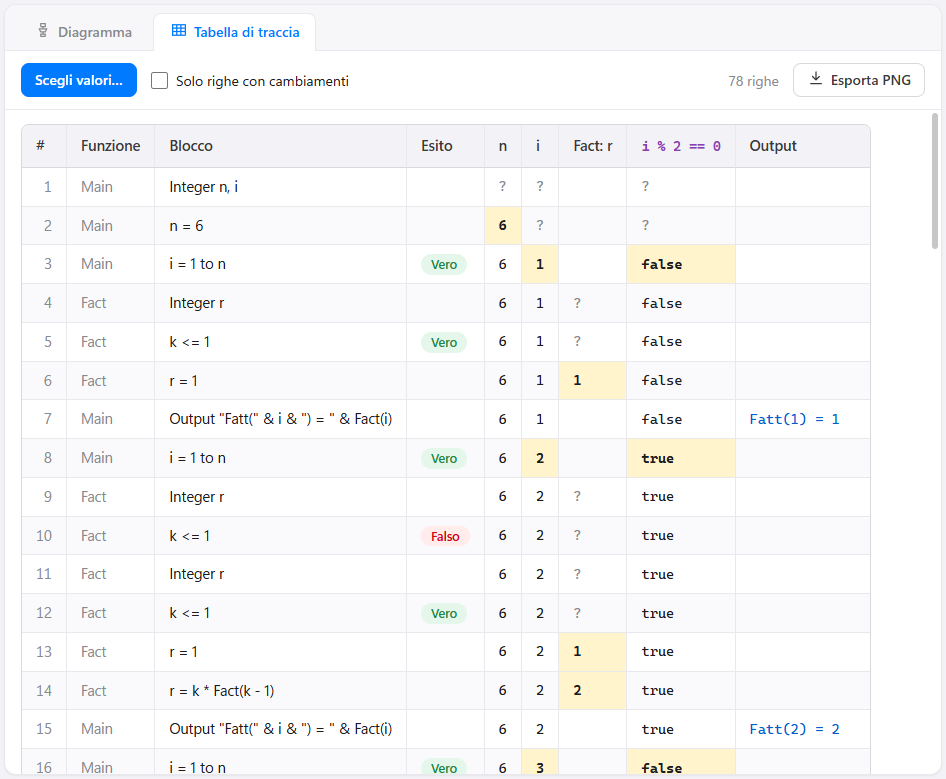
\includegraphics[width=0.95\linewidth]{trace-table.png}
  \caption{La tabella completa del programma Fattoriale, con la colonna Output.}
\end{figure}

% ==================== 11. FILE, SALVATAGGIO ED ESPORTAZIONE ====================
\section{File, salvataggio ed esportazione}

\subsection{Leggere e scrivere file}
I blocchi \textbf{Apri file}, \textbf{Leggi file}, \textbf{Scrivi file} e \textbf{Chiudi file} lavorano su file di testo, una riga per valore. Il nome del file è relativo alla cartella del programma salvato (o a Documenti, se il programma non è ancora salvato). \code{EOF()} dice quando il file è finito.

\begin{figure}[htbp]
  \centering
  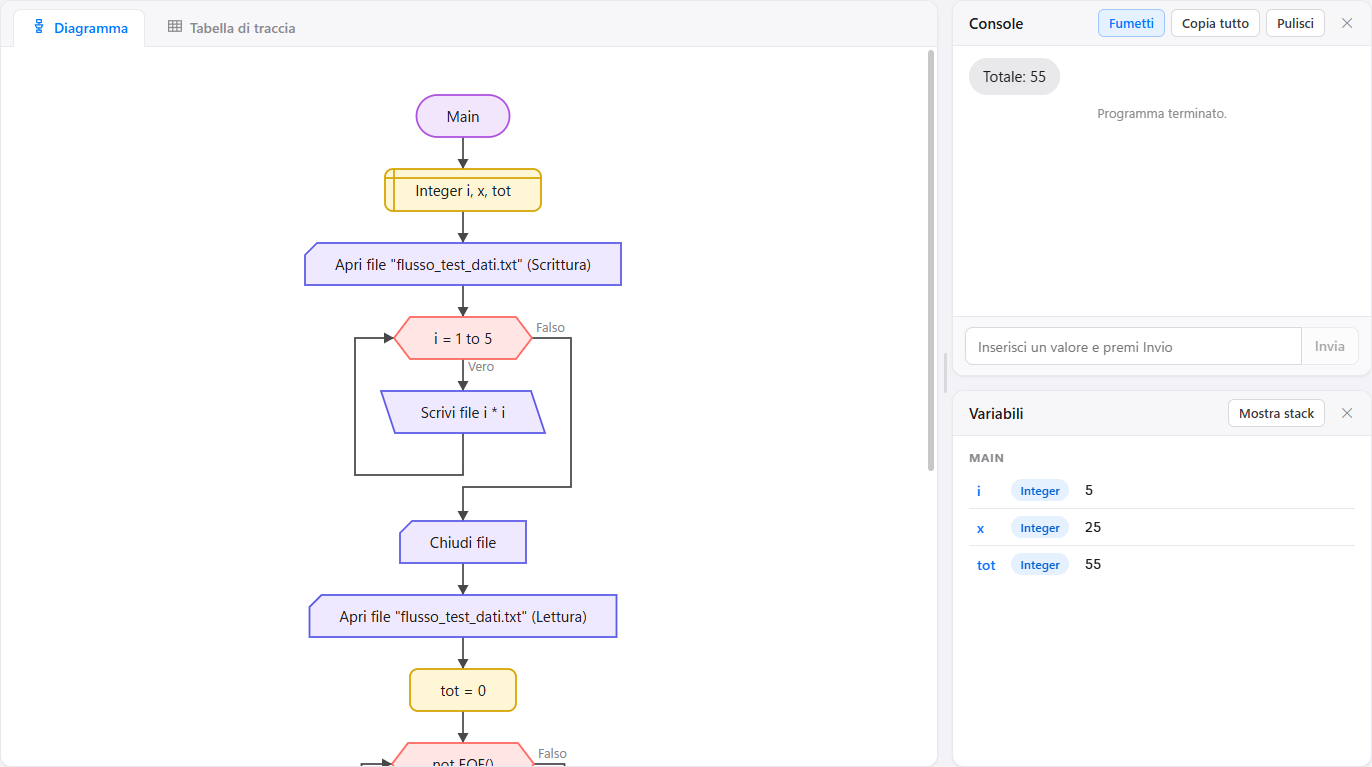
\includegraphics[width=0.95\linewidth]{files.png}
  \caption{L'esempio ``File'' scrive i quadrati da 1 a 25 e poi li rilegge sommandoli.}
\end{figure}

\subsection{Vedere il contenuto dei file}
Il pulsante \textbf{File} della barra apre il pannello omonimo, che mostra il contenuto dei file usati dal programma (quelli nominati nei blocchi \textbf{Apri file}). Si aggiorna mentre il programma gira, anche passo passo:
\begin{itemize}[label=\textcolor{ofPrimary}{$\checkmark$}, leftmargin=1.8em]
  \item in \textbf{lettura}, le righe già lette sono attenuate e la \textbf{prossima riga da leggere} è evidenziata;
  \item in \textbf{scrittura}, le righe compaiono man mano che vengono scritte (su disco vengono salvate alla chiusura del file);
  \item a programma fermo mostra il file com'è sul disco. Con \textbf{Apri\ldots} puoi vedere anche qualsiasi altro file di testo, per esempio per controllare i dati da leggere.
\end{itemize}

\begin{figure}[htbp]
  \centering
  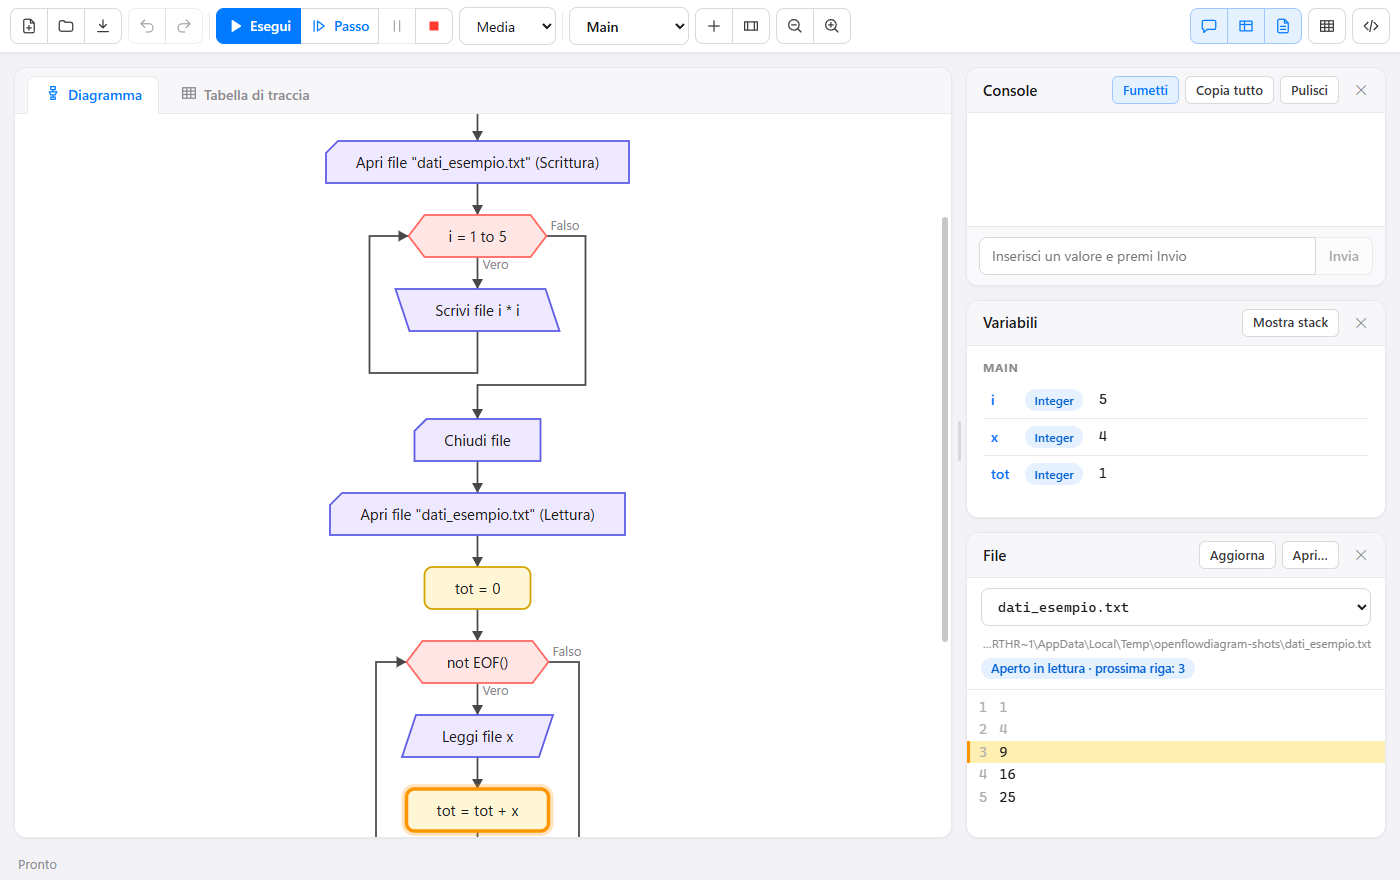
\includegraphics[width=0.95\linewidth]{file-viewer.png}
  \caption{Passo passo nell'esempio ``File'': le prime due righe sono già state lette (ora \code{x} vale 4) e nel pannello File è evidenziata la terza, la prossima che \textbf{Leggi file} leggerà.}
\end{figure}

\subsection{Salvare, aprire, esportare}
\begin{itemize}[label=\textcolor{ofPrimary}{$\checkmark$}, leftmargin=1.8em]
  \item \textbf{File \menuarrow{} Salva / Apri}: programmi in formato \code{.fprg}; puoi anche trascinare un file sulla finestra.
  \item \textbf{File \menuarrow{} Recenti}: gli ultimi file usati. \textbf{File \menuarrow{} Esempi}: programmi pronti (si aprono come copie senza nome).
  \item \textbf{File \menuarrow{} Esporta immagine PNG / SVG}: il diagramma della funzione mostrata.
  \item \textbf{File \menuarrow{} Stampa}: stampa tutte le funzioni, una per pagina.
  \item \textbf{Programma \menuarrow{} Attributi del programma}: nome, autori e descrizione salvati nel file.
\end{itemize}

% ==================== 12. PERSONALIZZARE ====================
\section{Personalizzare OpenflowDiagram}
Da \textbf{Strumenti \menuarrow{} Impostazioni} scegli lingua (italiano o inglese), schema colori, stile del diagramma, linguaggio predefinito per il codice e profondità massima delle chiamate.

\begin{figure}[htbp]
  \centering
  \begin{subfigure}[t]{0.48\linewidth}
    \centering
    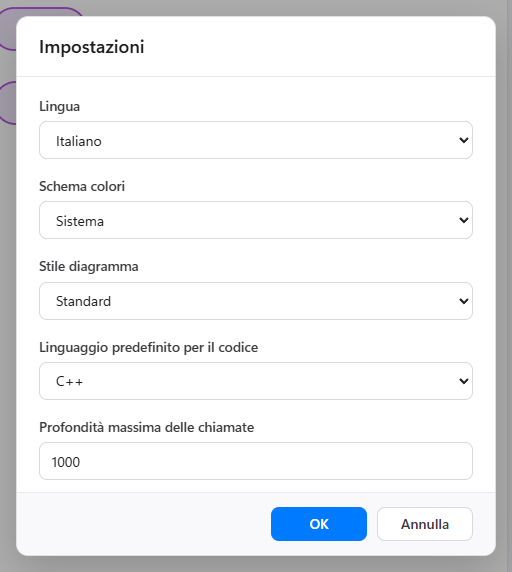
\includegraphics[width=\linewidth]{settings.png}
    \caption{Le impostazioni.}
  \end{subfigure}\hfill
  \begin{subfigure}[t]{0.48\linewidth}
    \centering
    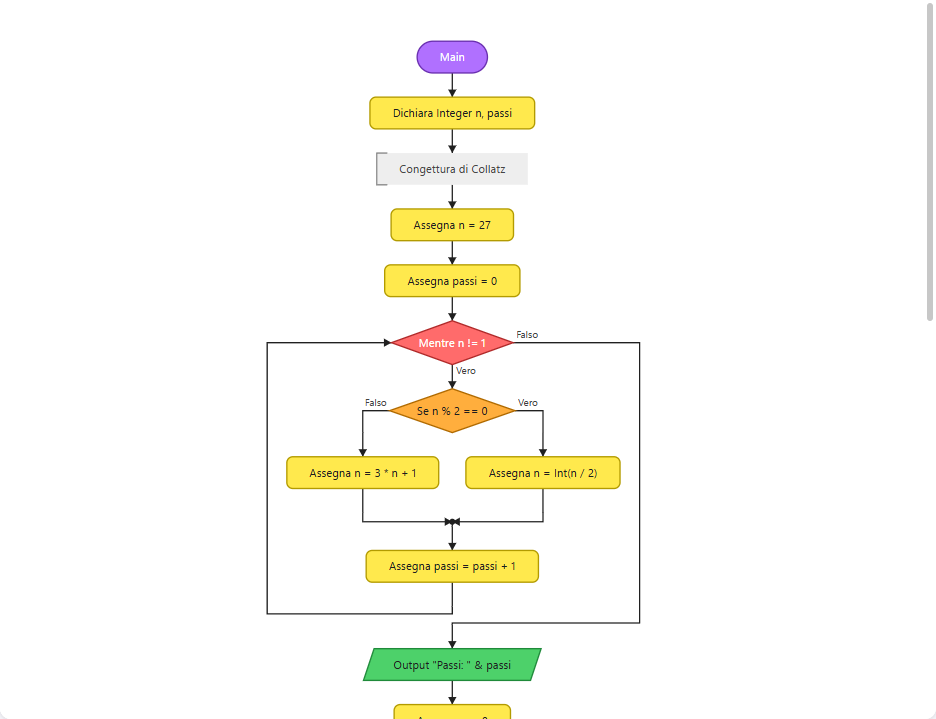
\includegraphics[width=\linewidth]{style-classic.png}
    \caption{Stile \textbf{Classico} con lo schema \textbf{Vivace}.}
  \end{subfigure}
\end{figure}

Schemi colore: \textbf{Sistema} (predefinito), Pastello, Vivace, Bianco e nero (adatto alla stampa), Progetto. Stili: \textbf{Standard}, \textbf{Descrittivo} (ogni blocco mostra anche il suo nome) e \textbf{Classico} (forme tradizionali). Si cambiano al volo anche da \textbf{Visualizza}.

% ==================== 13. SCORCIATOIE DA TASTIERA ====================
\section{Scorciatoie da tastiera}
\begin{longtable}{l p{10.5cm}}
  \toprule
  \textbf{Tasti} & \textbf{Azione} \\
  \midrule
  \endhead
  \bottomrule
  \endfoot
  \kbd{Ctrl}+\kbd{N} & Nuovo programma \\
  \kbd{Ctrl}+\kbd{O} & Apri \\
  \kbd{Ctrl}+\kbd{S} & Salva \\
  \kbd{Ctrl}+\kbd{Shift}+\kbd{S} & Salva con nome \\
  \kbd{Ctrl}+\kbd{P} & Stampa \\
  \kbd{Ctrl}+\kbd{Z} & Annulla \\
  \kbd{Ctrl}+\kbd{Y} & Ripeti \\
  \kbd{Ctrl}+\kbd{X} / \kbd{C} / \kbd{V} & Taglia, copia, incolla blocchi \\
  \kbd{Canc} & Elimina i blocchi selezionati \\
  \kbd{Invio} & Modifica il blocco selezionato \\
  \kbd{Esc} & Deseleziona / chiude una finestra \\
  \kbd{F5} & Esegui (o continua) \\
  \kbd{F10} & Passo \\
  \kbd{F6} & Pausa \\
  \kbd{Shift}+\kbd{F5} & Ferma \\
  \kbd{F4} & Mostra/nascondi il codice sorgente \\
  \kbd{F7} & Tabella di traccia \\
  \kbd{Ctrl}+\kbd{=} / \kbd{Ctrl}+\kbd{-} & Ingrandisci / riduci il diagramma \\
  \kbd{Ctrl}+\kbd{0} & Zoom 100\% \\
  \kbd{Ctrl}+\kbd{rotellina} & Zoom con il mouse \\
  \kbd{F1} & Questa guida (Aiuto \menuarrow{} Guida introduttiva) \\
\end{longtable}

% ==================== 14. ESEMPI ED ESERCIZI ====================
\section{Esempi ed esercizi}
In \textbf{File \menuarrow{} Esempi} trovi:

\begin{tabularx}{\linewidth}{>{\bfseries}l X}
  \toprule
  Esempio & \textbf{Cosa mostra} \\
  \midrule
  Fattoriale & ciclo Per e funzione ricorsiva \\
  Ordinamento & array, funzioni con parametri array (bubble sort e somma) \\
  Cicli & Mentre, Ripeti, Per decrescente, Se annidati, breakpoint \\
  Input & lettura di testi, numeri e valori Boolean \\
  Stringhe & Len, Char, ToCode, ToChar, confronti tra testi \\
  File & scrittura e lettura di un file di testo \\
  \bottomrule
\end{tabularx}

\subsection{Esercizi per iniziare}
\begin{enumerate}[leftmargin=1.8em]
  \item \textbf{Pari o dispari} --- chiedi un numero e scrivi se è pari o dispari (suggerimento: \code{n \% 2 == 0}).
  \item \textbf{Tabellina} --- chiedi un numero e stampa la sua tabellina da 1 a 10 con un ciclo Per.
  \item \textbf{Indovina il numero} --- il programma sceglie \code{Random(100) + 1} e risponde ``più alto'' o ``più basso'' finché non indovini (ciclo Ripeti).
  \item \textbf{Media dei voti} --- leggi 5 voti in un \code{Real Array} e calcola la media; usa \code{ToFixed(media, 2)} per l'output.
  \item \textbf{Massimo con funzione} --- scrivi una funzione \code{Massimo(Integer Array a)} che restituisce il valore più grande e seguila con la tabella di traccia.
\end{enumerate}

% ==================== 15. DOMANDE FREQUENTI ====================
\section{Domande frequenti}
\begin{description}[style=nextline, leftmargin=0pt, itemsep=6pt]
  \item[Il programma non parte e un blocco è tratteggiato.]
    Il blocco è incompleto: fai doppio clic e compila i campi.
  \item[«La variabile \ldots\ non è stata inizializzata».]
    La variabile è dichiarata ma non ha ancora un valore: assegnale un valore o leggila con Input prima di usarla.
  \item[«Tipo del valore incompatibile».]
    Stai mettendo, per esempio, un Real in una variabile Integer: usa \code{Int(\ldots)} o dichiara la variabile Real.
  \item[Il programma non finisce mai.]
    Probabilmente un ciclo infinito: premi \textbf{Ferma} e controlla che la condizione del ciclo possa diventare falsa.
  \item[Voglio vedere un ciclo lentamente.]
    Scegli la velocità \textbf{Lenta}, oppure usa \textbf{Passo} e la tabella di traccia.
  \item[Come cambio lingua?]
    \textbf{Strumenti \menuarrow{} Impostazioni \menuarrow{} Lingua} (Tools \menuarrow{} Settings in inglese).
\end{description}

\vfill
\begin{center}
  \small\textcolor{ofMuted}{OpenflowDiagram 1.0.0 \textperiodcentered\ Guida introduttiva}
\end{center}

\end{document}
